\documentclass[12pt, a4paper, titlepage]{report}
\usepackage{graphicx, amsmath, amsfonts, listings, amssymb, mathrsfs, color, fancyhdr, geometry, hyperref}
\usepackage[english]{babel}
\usepackage[utf8x]{inputenc}
\usepackage{wrapfig}
\graphicspath{ {images/} }

\geometry{
a4paper,bindingoffset=0.2in,
            left=1in,right=1in,top=1in,bottom=1in,
            footskip=.25in
 }
\definecolor{mygreen}{RGB}{28,172,0}
\definecolor{mylilas}{RGB}{170,55,241}
\pagestyle{fancy}
\fancyhf{}
\rhead{Ashish T., Nischal L.S., Sagar D.}
\lhead{Election Portal}
\fancyfoot[C]{Page \thepage}
\renewcommand{\headrulewidth}{2pt}

\begin{document}


\begin{titlepage}
\newcommand{\HRule}{\rule{\linewidth}{0.5mm}}
\center
\begin{center}
	
\includegraphics[scale=0.4]{ncit}
\end{center}
\vspace{0.75cm}
 \textsc{\Large \textbf{Nepal College of Information Technology}}\\
{\large \textbf{Web Design Competition} \par}
\vfill
\HRule \\[0.4cm]

\includegraphics[scale=0.4]{logo.png}\\[1cm] 
{ \huge \bfseries Election Portal}\\
\textsc{\large Discover everything election!}
\HRule \\[1.5cm]
\vfill
{\large Team members}\\
{\Large \textbf{Ashish Tiwari} \par}
{\Large \textbf{Nischal Lal Shrestha} \par}
{\Large \textbf{Sagar Devkota} \par}
\vfill
{\large \today}\\[1cm] 
\end{titlepage}


\begin{abstract}
The purpose of Election Portal is to digitize election and election-related activities in Nepal. Election Portal offers a web application to store candidates information, election constituency details, latest election results. The problem statement relies on understanding a way to store all the dataset in the database, solving the complexity involved within and finding an interface to provide all these dataset to the visitors without a pain. Election Portal will provide opportunity to individual volunteers to update the election datasets election result in real time. Each web page of the Election Portal will be equipped with either a search form or a filter form to enhance user's ability to get information very quickly.
\end{abstract}

\section{Introduction}
Election Portal is a web application for individual visitors, journalists, students to get election results and other election-related activities at a single place. Election Portal will provide oppurtunity to individual volunteers to update the election datasets, election result in a real time.

\section{Problem Statement}
The problem statement for Election Portal is based on understanding and developing a effective way to store all the datasets of election-related activites in a profound way, solving all the complexity involved with the datasets. It also relies on building a interface to filter and search the election datasets through the database in a effective manner.

\newpage
\section{UML Design}
\subsection{Use Case Diagram}
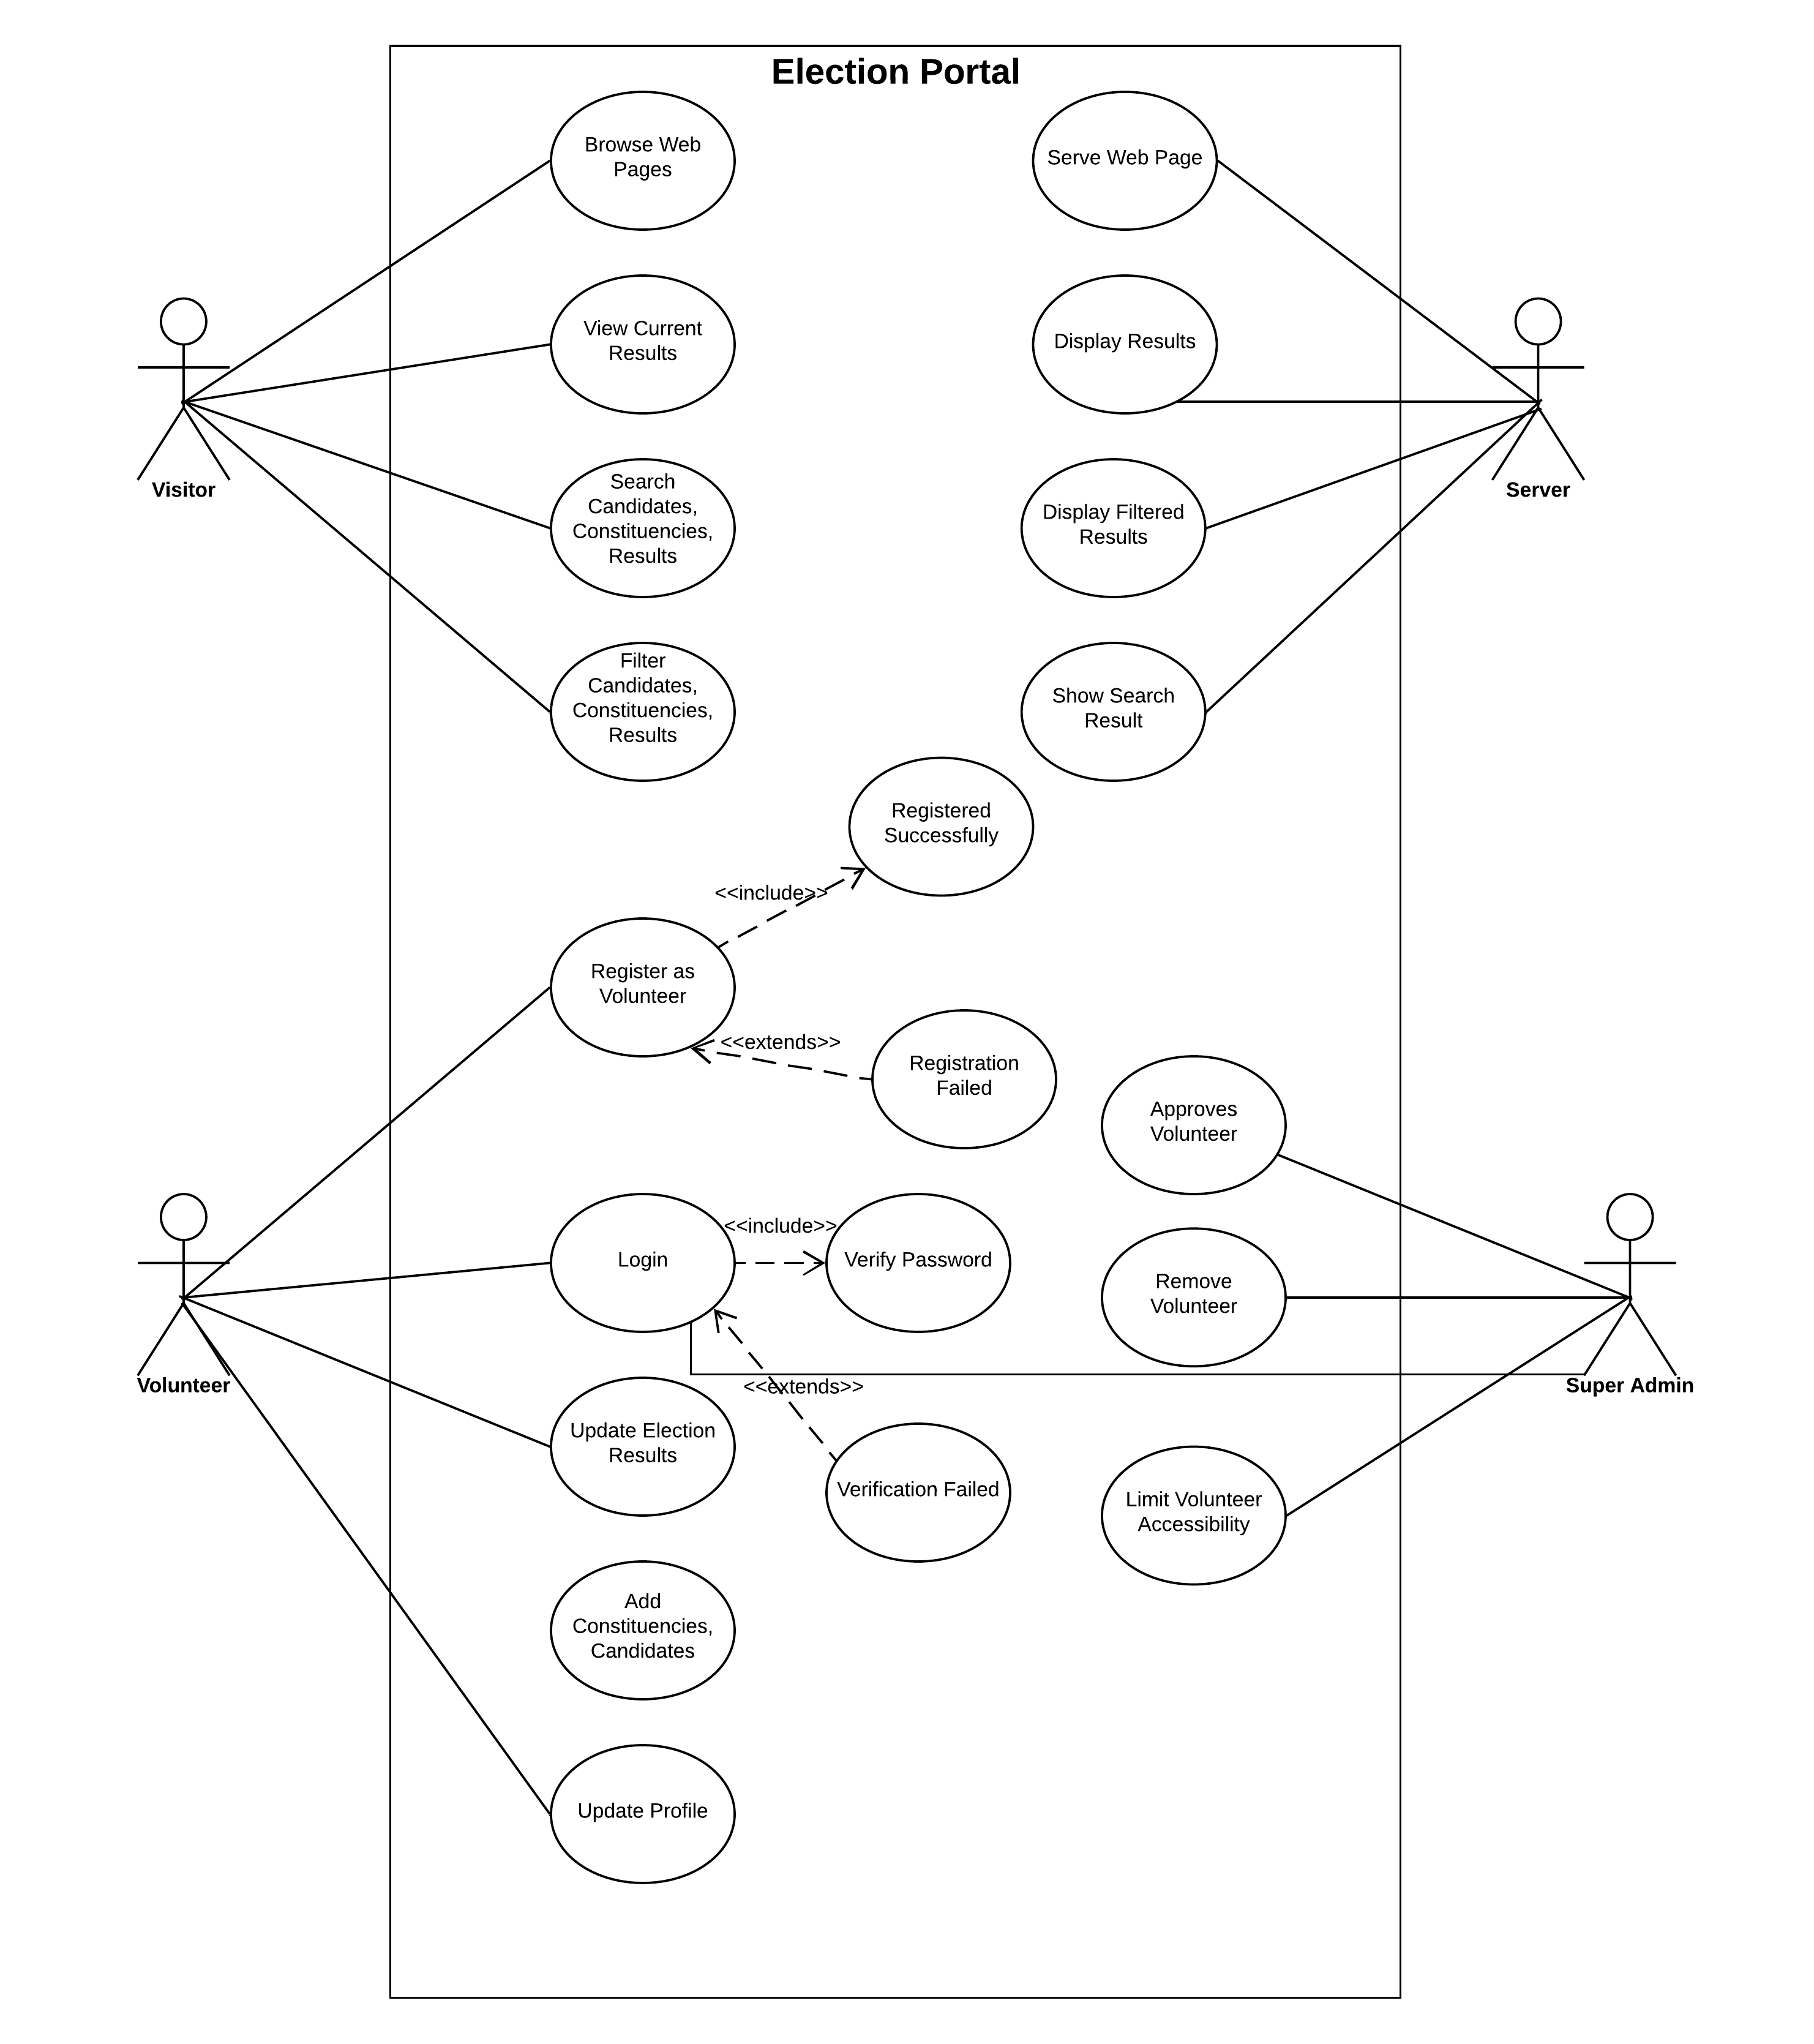
\includegraphics[scale=0.6]{election_portal_use_case_diagram.png}\\

The Use Case Diagram of Election Portal contains the scope of the system. It lists all the functionalites offered by the system. We had identified following actors:
\begin{enumerate}
\item Visitor:- Visitor represents as the primary actor for this system. Vistors can browse web pages, view current results, search and filter candidates, constituencies, results.

\item Volunteer:- Volunteer act to update election results, add new datasets in the system. Volunteer needs to register first and then login to make changes in the system.

\item Super Admin:- Super Admin regulates the database. Super Admin approves new volunteer, remove volunteer and limit their access to the database.

\item Server:- A Server act to store the volunteers authentications information. Server acts to provides the web pages and datasets from database to users on their requests throuh a web browser. 
\end{enumerate}

Based on the above Use Case Diagram we can identify the following group of activities:

\begin{enumerate}
\item Visitors enters the web portal and browse various web pages.

\item Visitors can either search or filter the datasets through form.

\item Volunteer can Create, Read, Update and Delete datasets from the database.

\item Super Admin can approve new volunteer, limit access to volunteer and delete existing volunteer.
\end{enumerate}
\subsection{UML Class Diagram}
\begin{center}
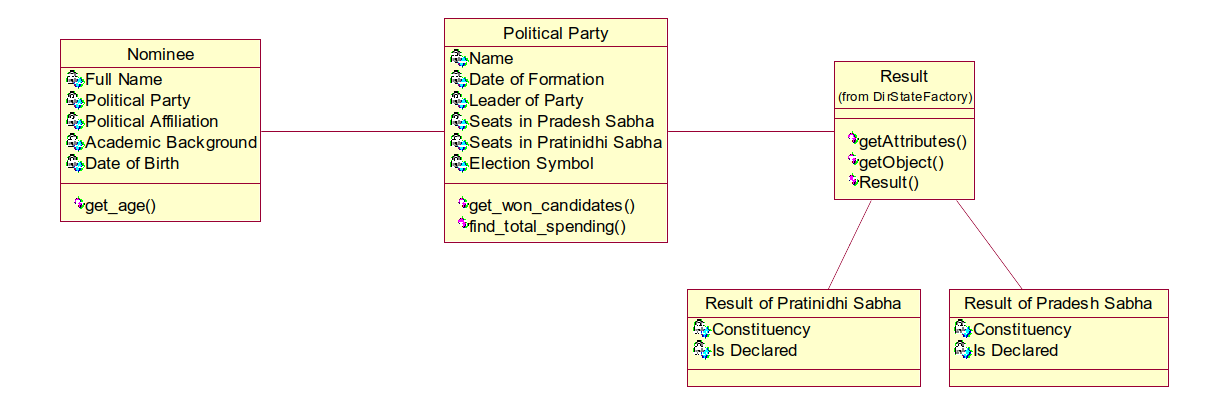
\includegraphics[scale=0.5]{political_party.png}

\end{center}

\begin{center}
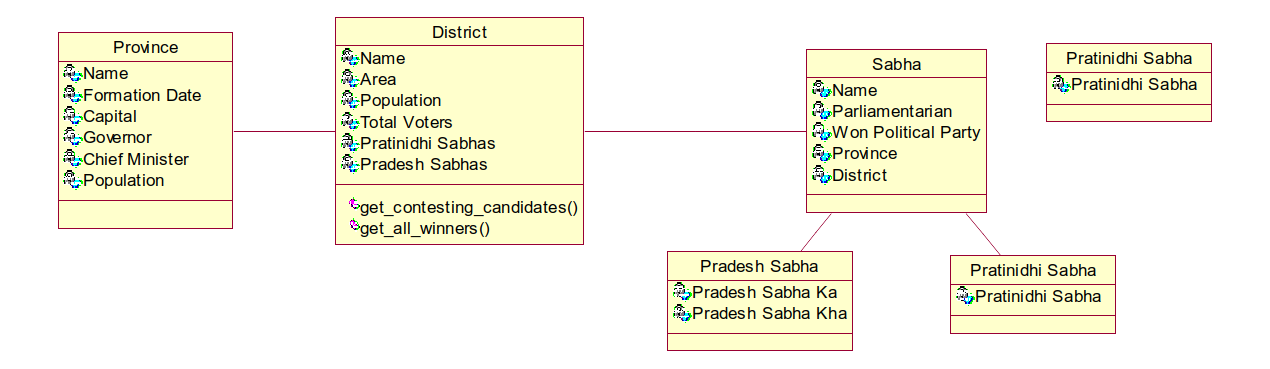
\includegraphics[scale=0.5]{Political_division.png}
\end{center}


\section{Framework of the Development}
\subsection{Logical Architecture Diagram}
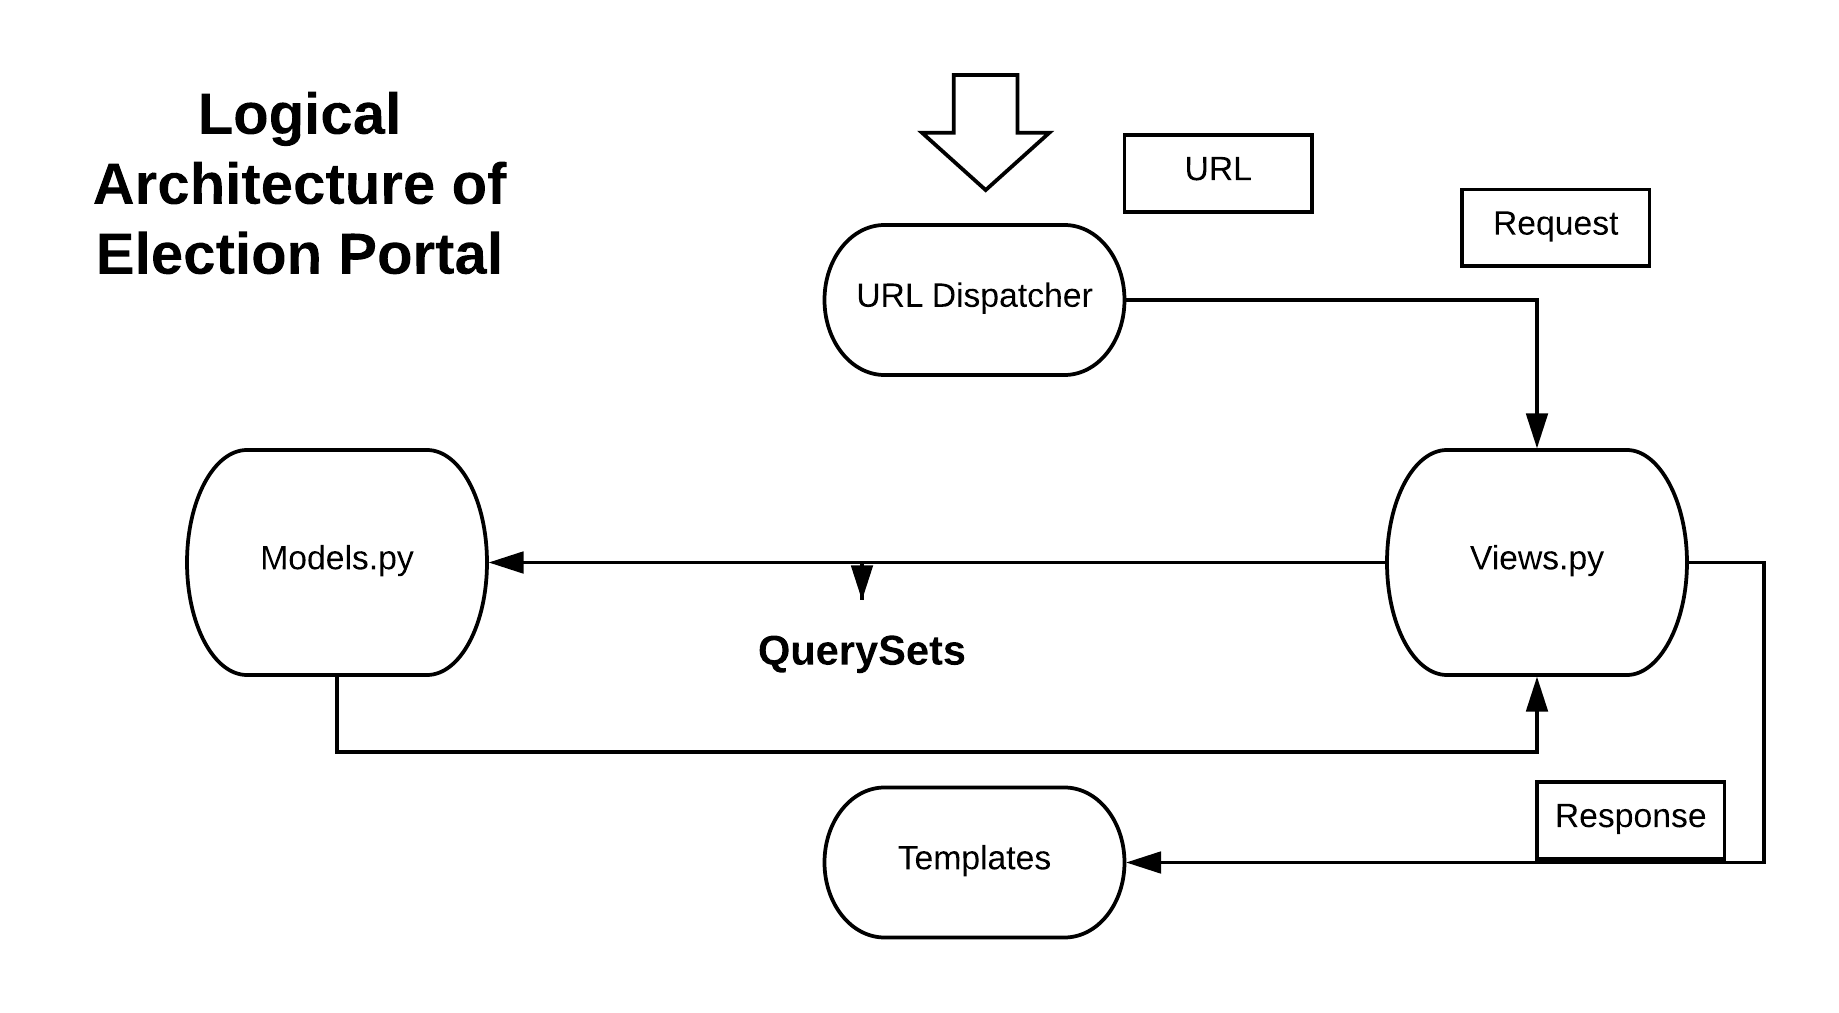
\includegraphics[scale=0.8]{Logical_Architecture.png}\\
There are three layers between User Interface and Database. Those are:
\begin{enumerate}
\item Data Access Layer(models.py)\\
This layers defines everything about the data: how to access data, how we can validate data, what type of behaviors our data will show, and what type of relationship exists between different data.
\item Presentation Layer(Templates)\\
Presentation layer will define how something should be displayed on a Web Page. Presentation layer takes information from the database and display it to the user in a Human-Understandable-Format. Presentation layer is completely free of any king of logic.
\item Business Logic Layer(views.py)\\
Business Logic Layer is a bridge between models and templates. It provides appropriate way to supply specific templates requested by the data access layer.
\end{enumerate}
\newpage

\section{Tools and Technology Used}

\begin{enumerate}
\item Django:- Django is a high-level Python Web framework that encourages rapid development and clean, pragmatic design. Built by experienced developers, it takes care of much of the hassle of Web development, so you can focus on writing your app without needing to reinvent the wheel. It’s free and open source

\item 
U.S. Web Design System:- 
A design system for the federal government

Design and build fast, accessible, mobile-friendly government websites backed by user research.


\item SQLite:- SQLite is a self-contained, high-reliability, embedded, full-featured, public-domain, SQL database engine. SQLite is the most used database engine in the world.

\item JQuery:- JQuery is a fast and concise JavaScript Library created by John Resig in 2006 with a nice motto: Write less, do more. jQuery simplifies HTML document traversing, event handling, animating, and Ajax interactions for rapid web development.

\item Html and CSS:- HTML, HyperText Markup Language, gives content structure and meaning by defining that content as, for example, headings, paragraphs, or images. CSS, or Cascading Style Sheets, is a presentation language created to style the appearance of content—using, for example, fonts or colors.
\end{enumerate}
\newpage
\section{Installation}
\subsection{Installing Python}

Election Portal is a django app. Django is written in 100 percent pure Python code, so you’ll need to install Python on your system. Django requires Python 2.3 or higher.
If you’re on Linux or Mac OS X, you probably already have Python installed.

\subsection{Creating an isolated Python environment}
A virtual environment (also called a virtualenv) is like a private box where we can stuff useful computer code into for a project
we're working on It is recommended that you use virtualenv to create isolated Python environments, so you can use different package versions for different projects, which is far more practical than installing Python packages system wide.

To install virtualenv:
\begin{center}
pip install virtualenv
\end{center}
    

After you install virtualenv, create an isolated environment with the following command:

\begin{center}
virtualenv myenvironment
\end{center}

    

Note: Here `myenvironment' can by any valid name you like.

Now, You created a virtual environment let's activate it:

To Activate:
\begin{center}
source myenvironment/bin/activate
\end{center}

\subsection{Requirements.txt}
This file consist all the dependencies of this app.\\
Our web app need following packages to work correctly:\\
chardet==3.0.4\\
Django==2.0.7\\
doc8==0.8.0\\
docutils==0.14\\
pbr==4.0.4\\
pkg-resources==0.0.0\\
pytz==2018.5\\
restructuredtext-lint==1.1.3\\
six==1.11.0\\
stevedore==1.28.0\\

To install all the dependencies, just type:

\begin{center}
pip install -r Requirements.txt
\end{center}
    
   
Make Sure You have an active internet connection.

Now, All our dependencies are fullfilled.

In your terminal, Change Directory to the Base Directory of our website. i.e the folder which consist manage.py:

\begin{center}
cd ElectionPortalWebapp
\end{center}

    
    
Then:
\begin{center}
    python manage.py collectstatic\\
    python manage.py makemigrations\\
    python manage.py migrate\\
\end{center}




To Run The Server:

\begin{center}
python manage runserver
\end{center}

Our web app is ready for local development.
    
\newpage
    
\section{Graphical User Interface of the System}
Election Portal has a GUI so that visitors can easily browse the portal with the least effort. Every page has a header and footer. The header consists of the Navigation menu so that visitors can navigate throughout the webpage without being lost.
\subsection{Homepage}
\begin{center}
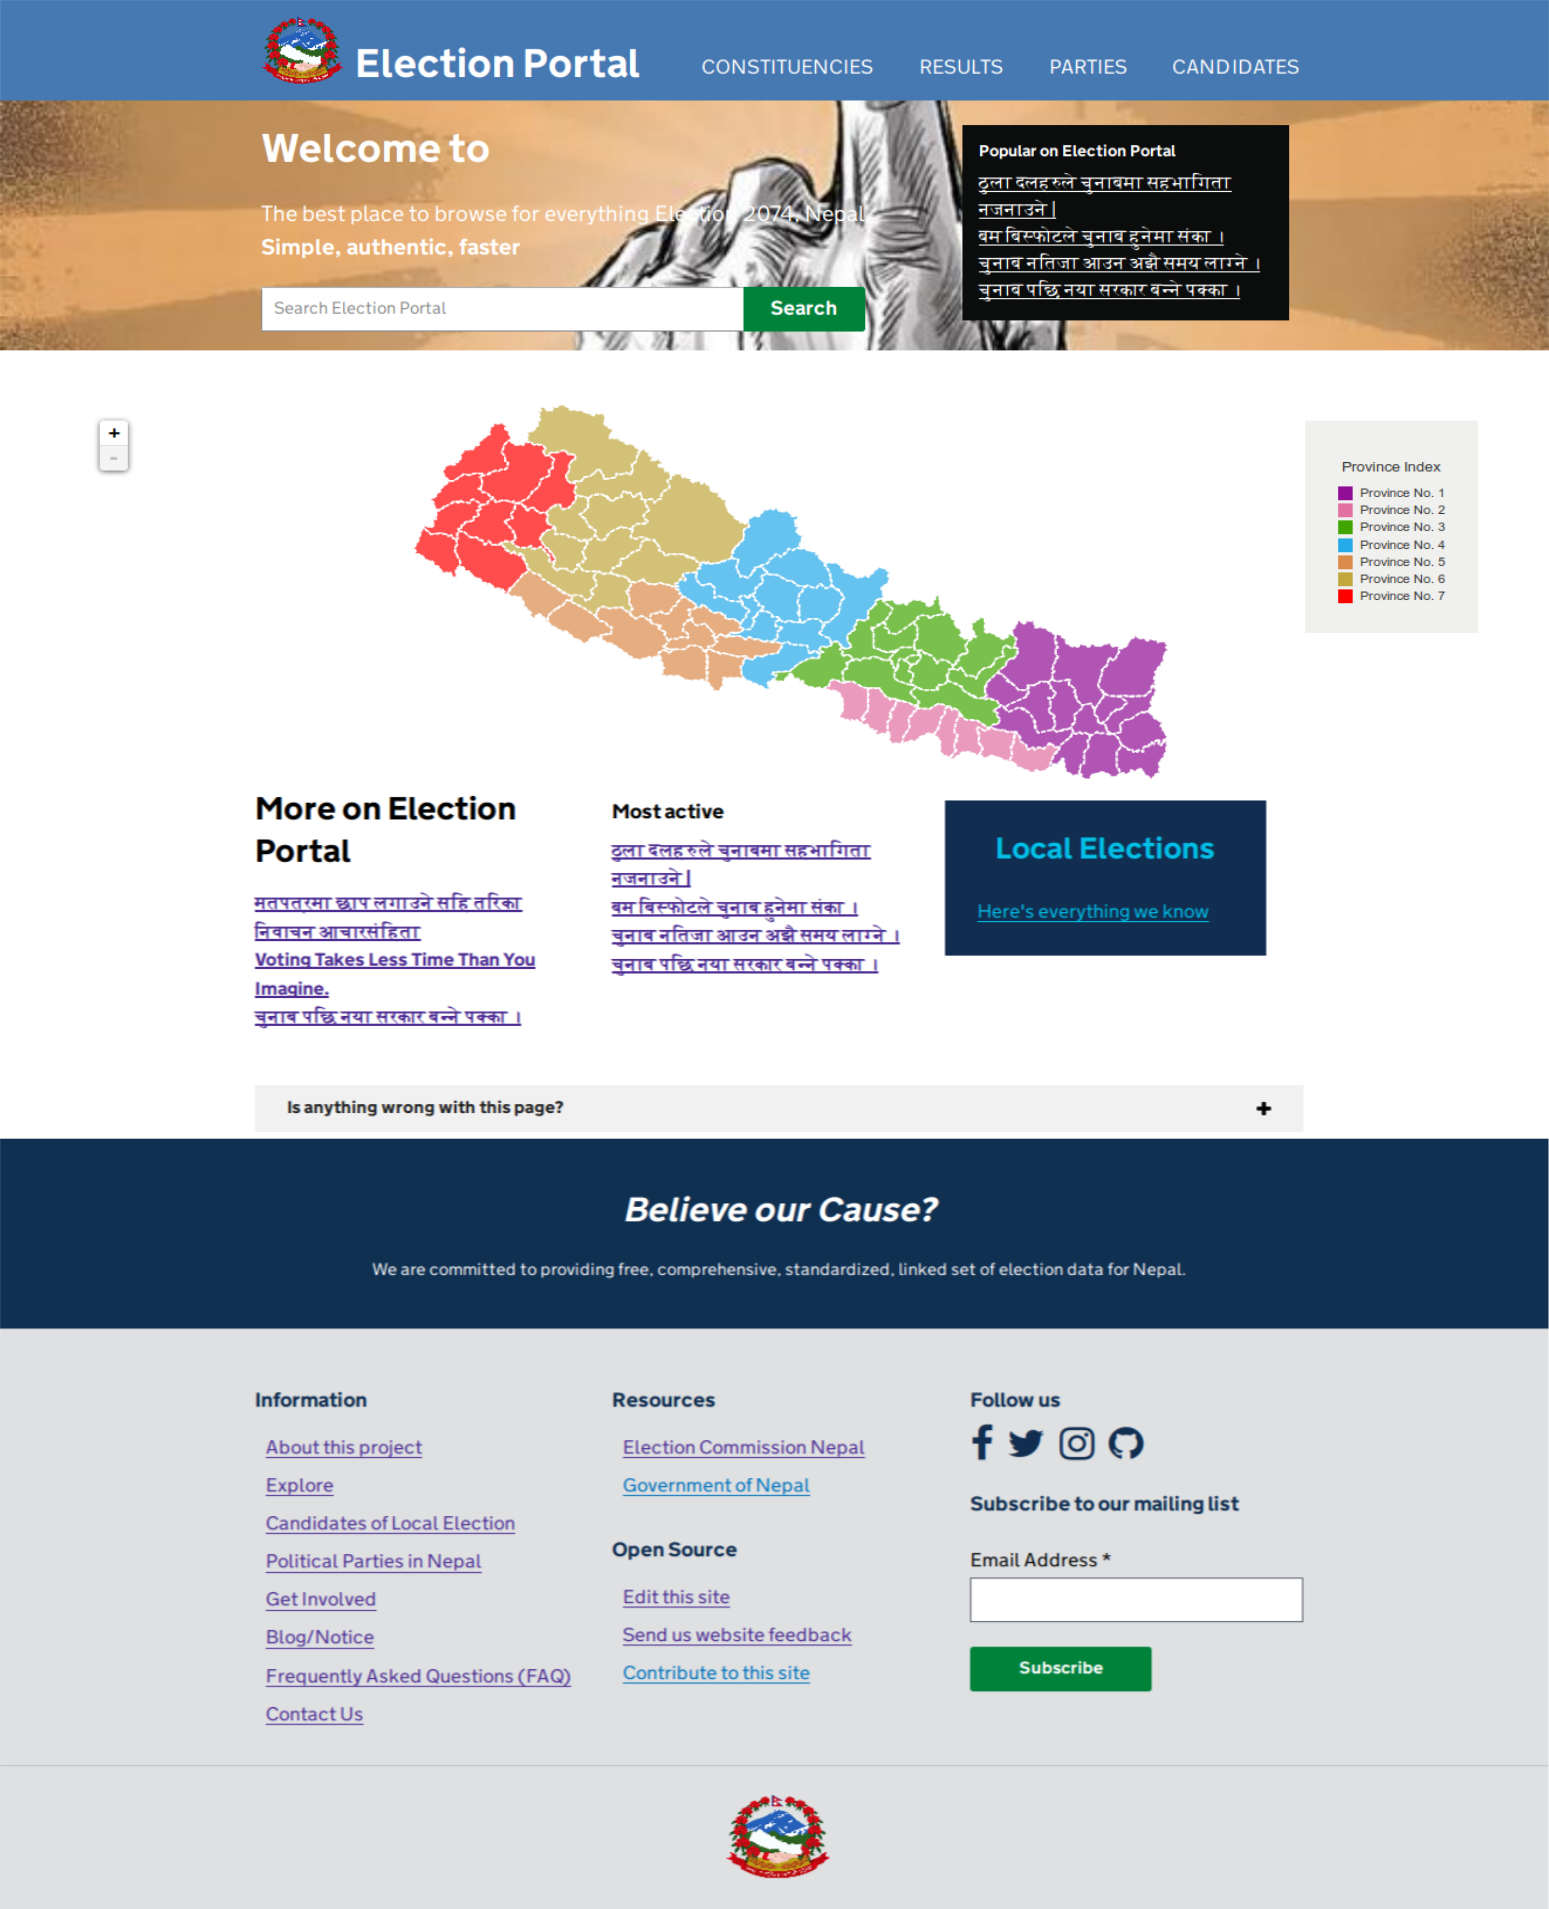
\includegraphics[scale=0.25]{Homepage.png}\\
\end{center}

Beside Header and Footer, Homepage of Election Portal has a search form which allows visitors to search election datasets without a pain. The homepage has a map, so any users can filter the datasets via district.
\newpage
\subsection{List of Political Party}
All the political parties registered will be listed here along with their party image. Given figure shows same image because we don't have update the database with real datas.\\
\begin{center}
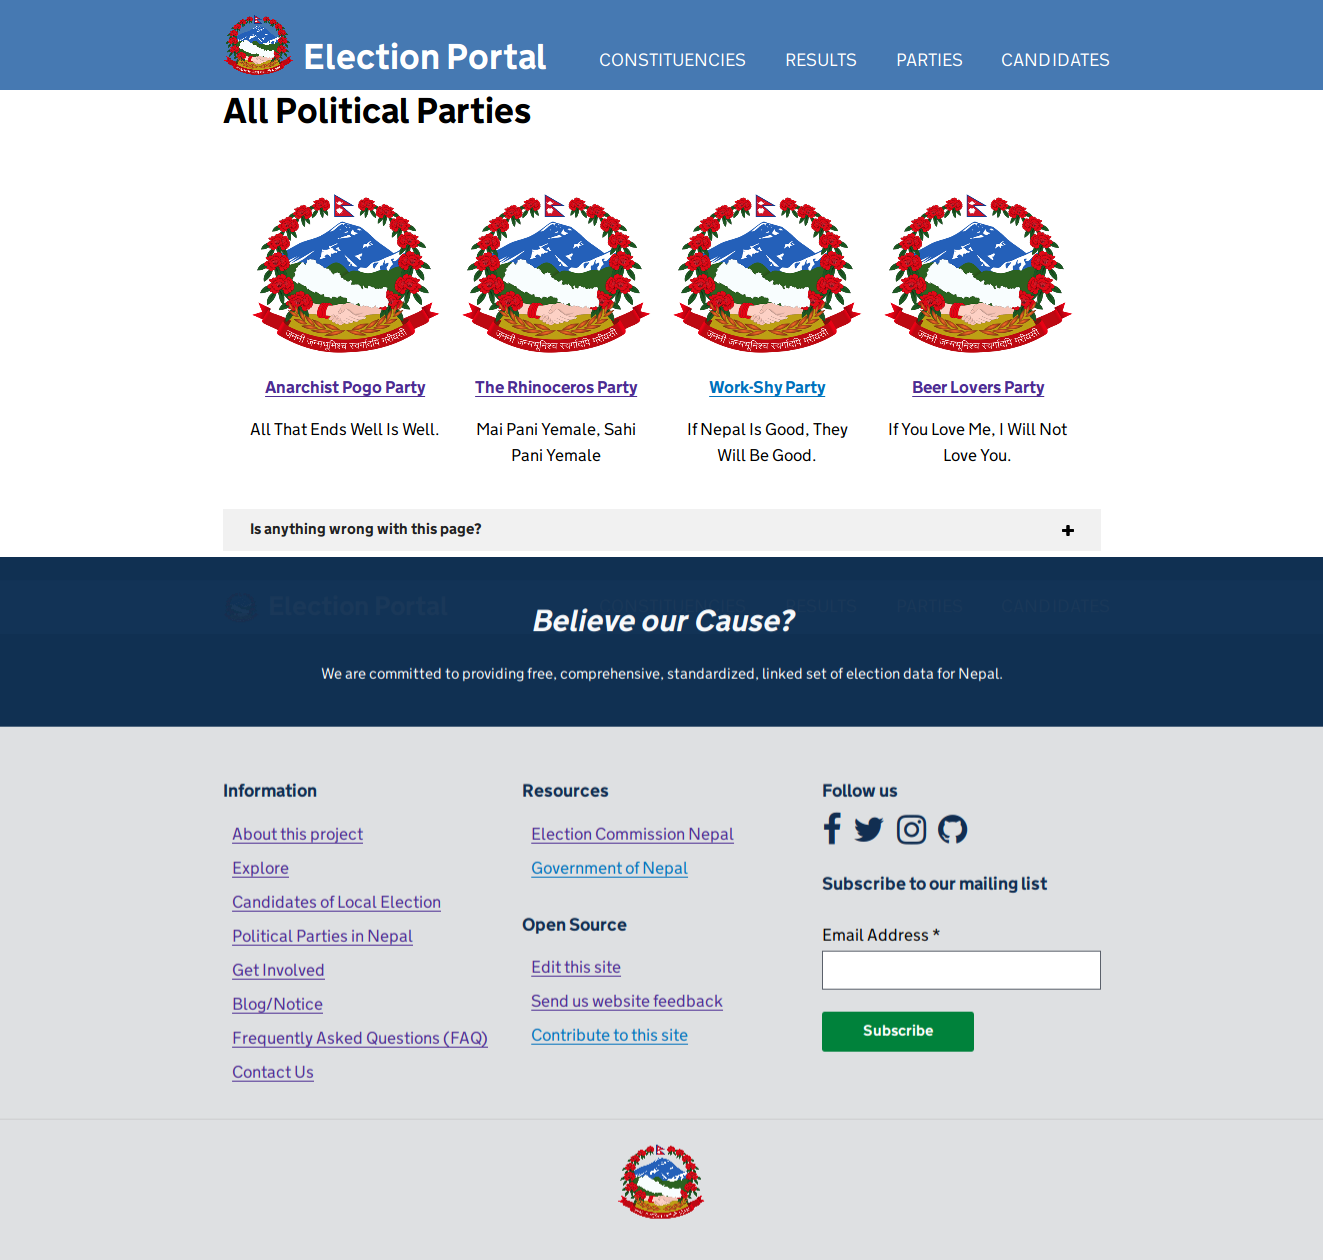
\includegraphics[scale=0.25]{List_of_Political_Party.png}\\
\end{center}

\newpage
\subsection{Details of Political Party}
\begin{center}
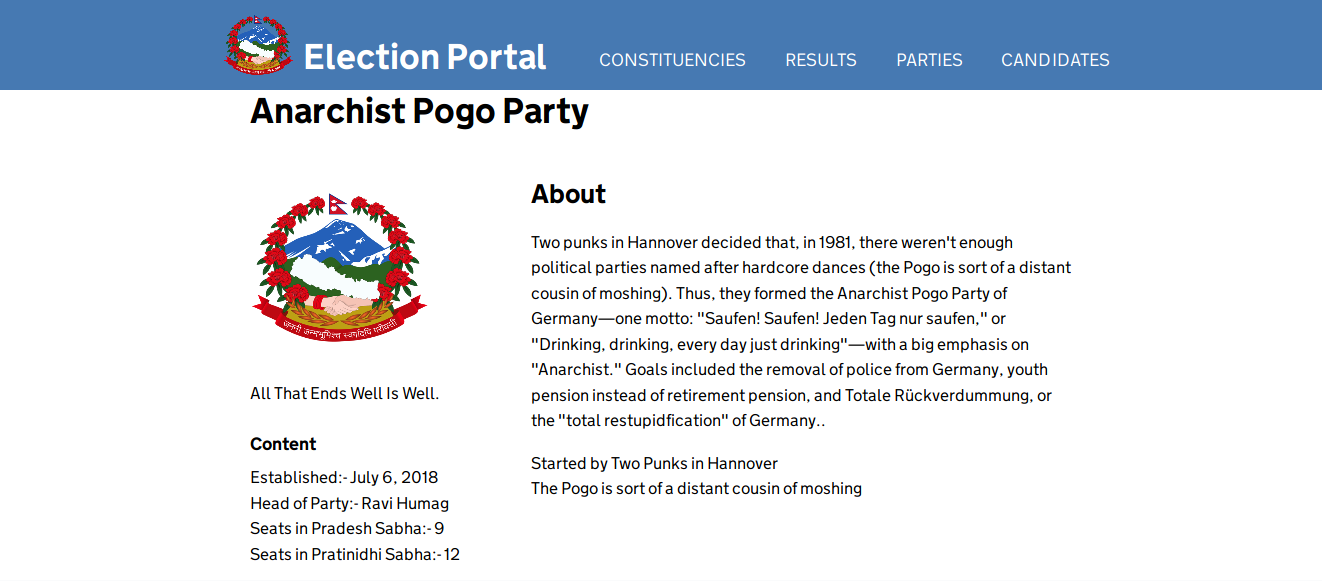
\includegraphics[scale=0.25]{Details_of_Political_Party.png}
\end{center}

\subsection{Details of Nominee}
\begin{center}
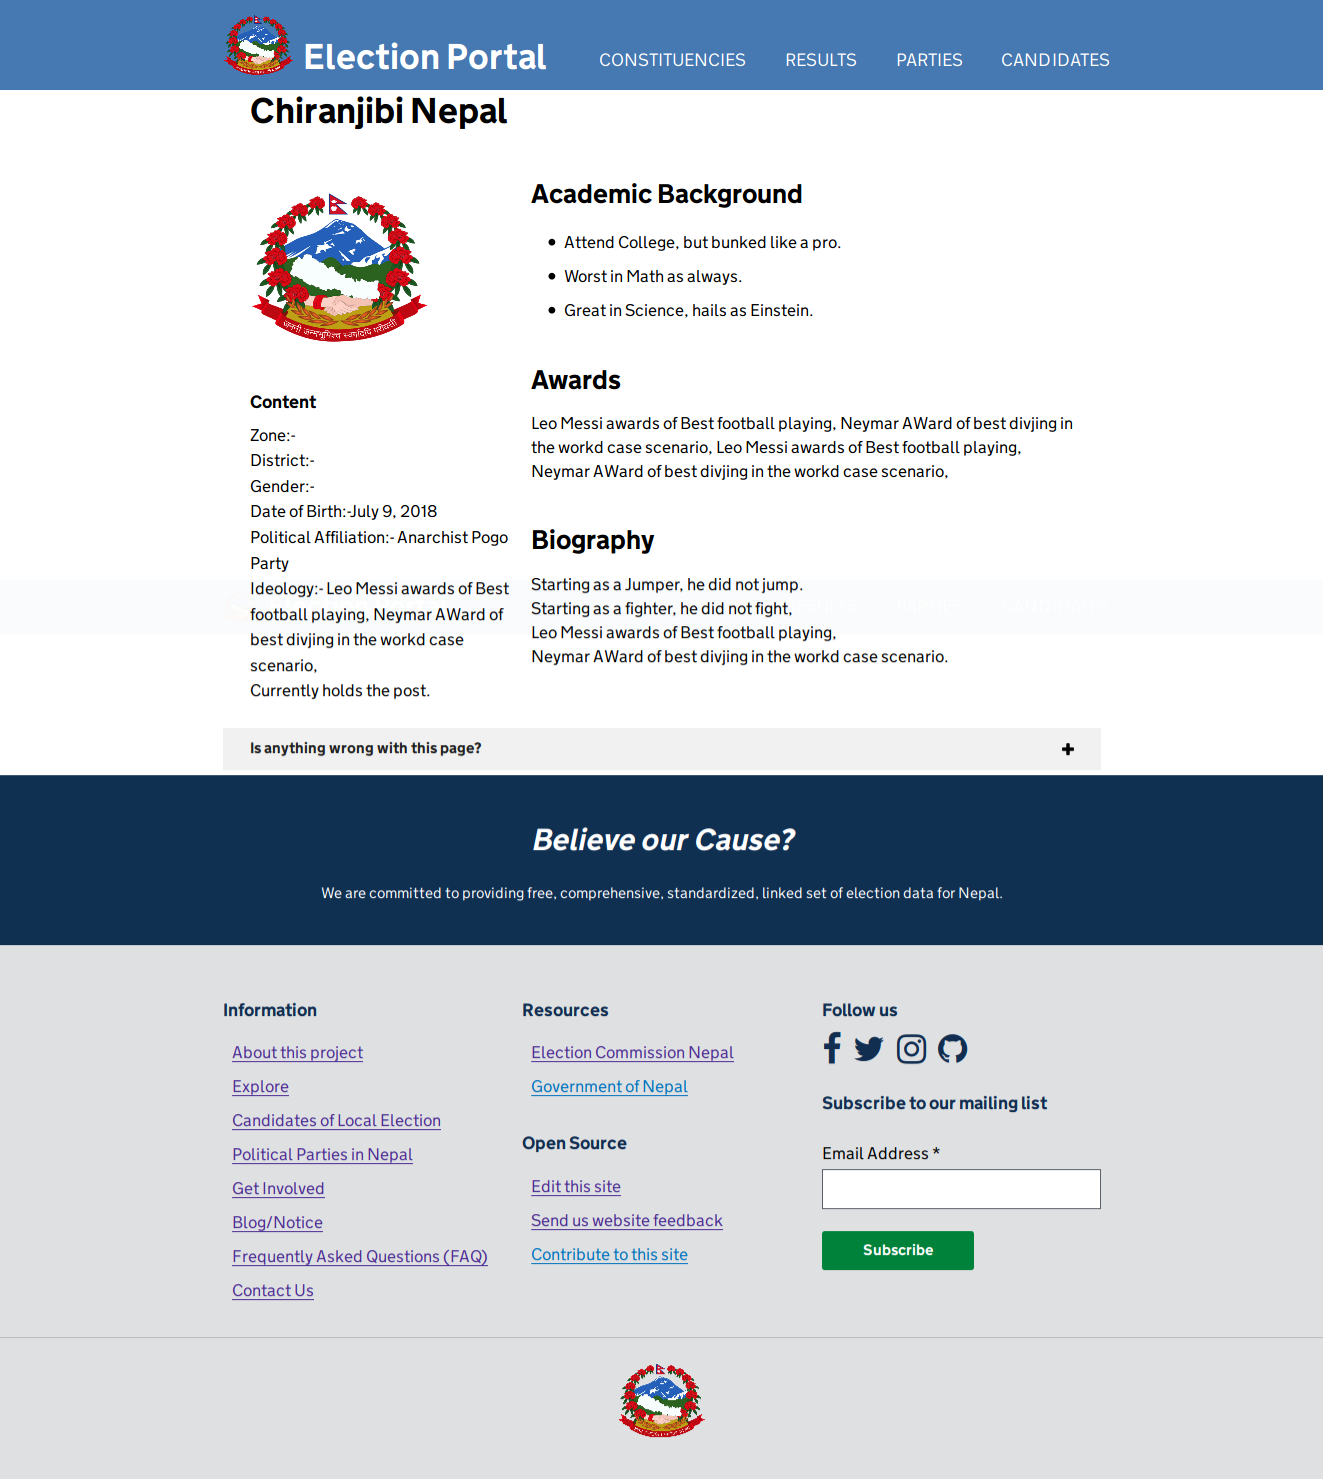
\includegraphics[scale=0.25]{Details_of_a_nominee.png}
\end{center}


\subsection{Details of Constituency}
\begin{center}
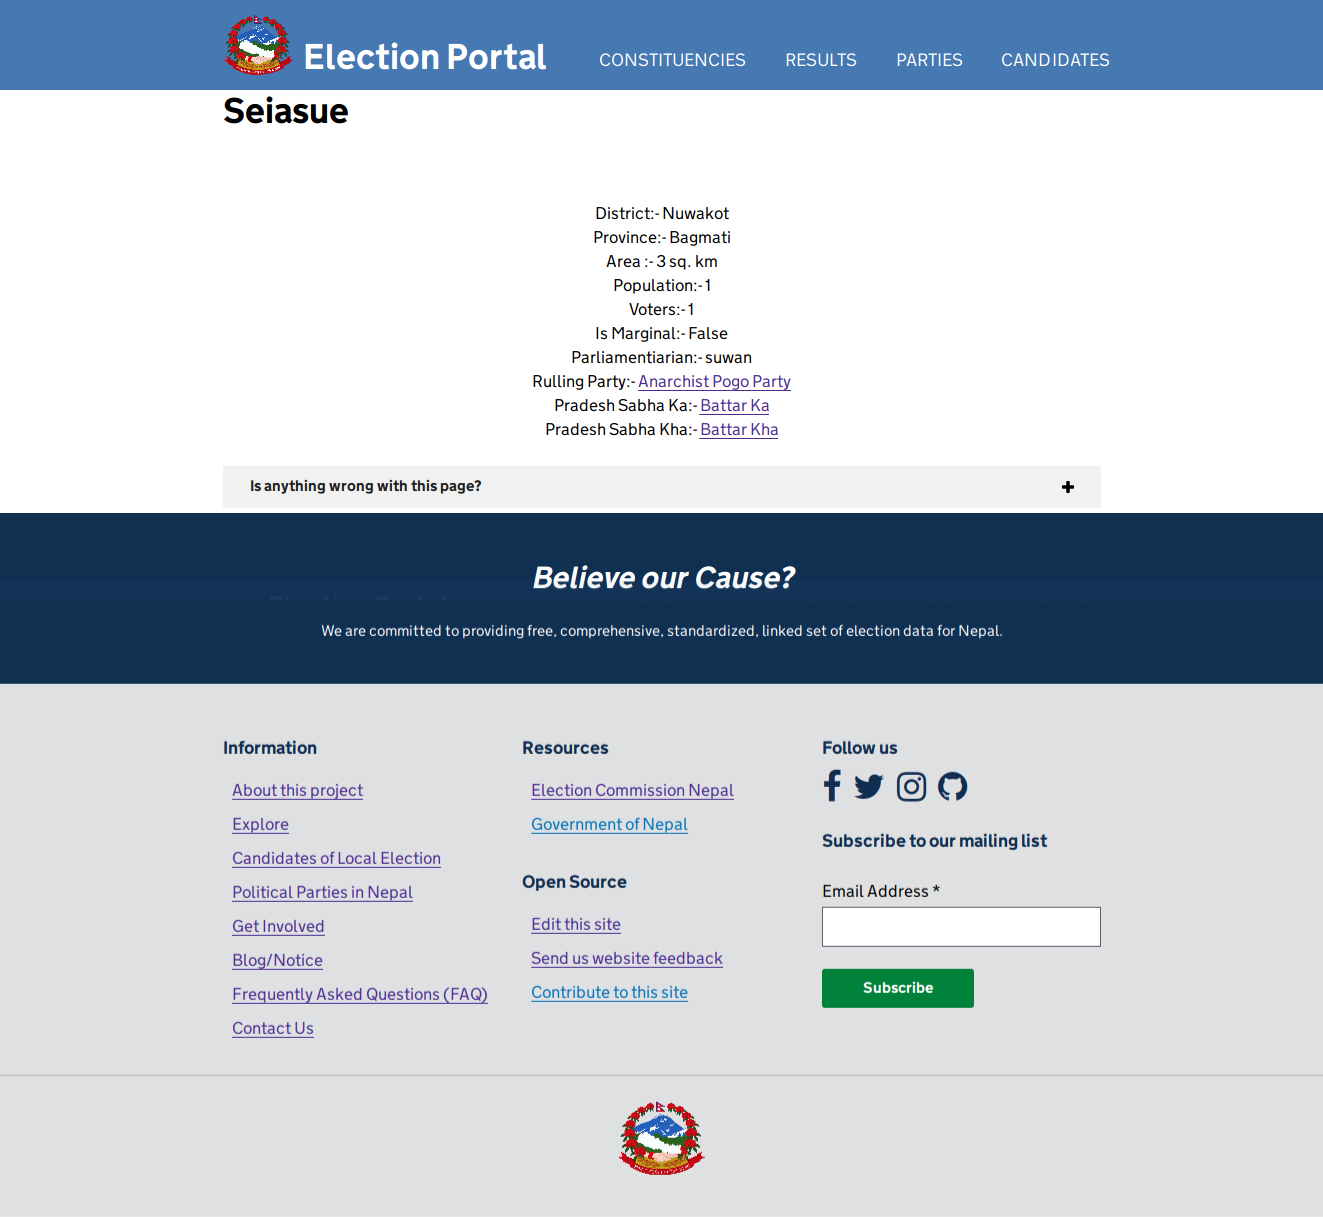
\includegraphics[scale=0.25]{Details_of_Constituency.png}
\end{center}


\subsection{Form to Add Nominee}
\begin{center}
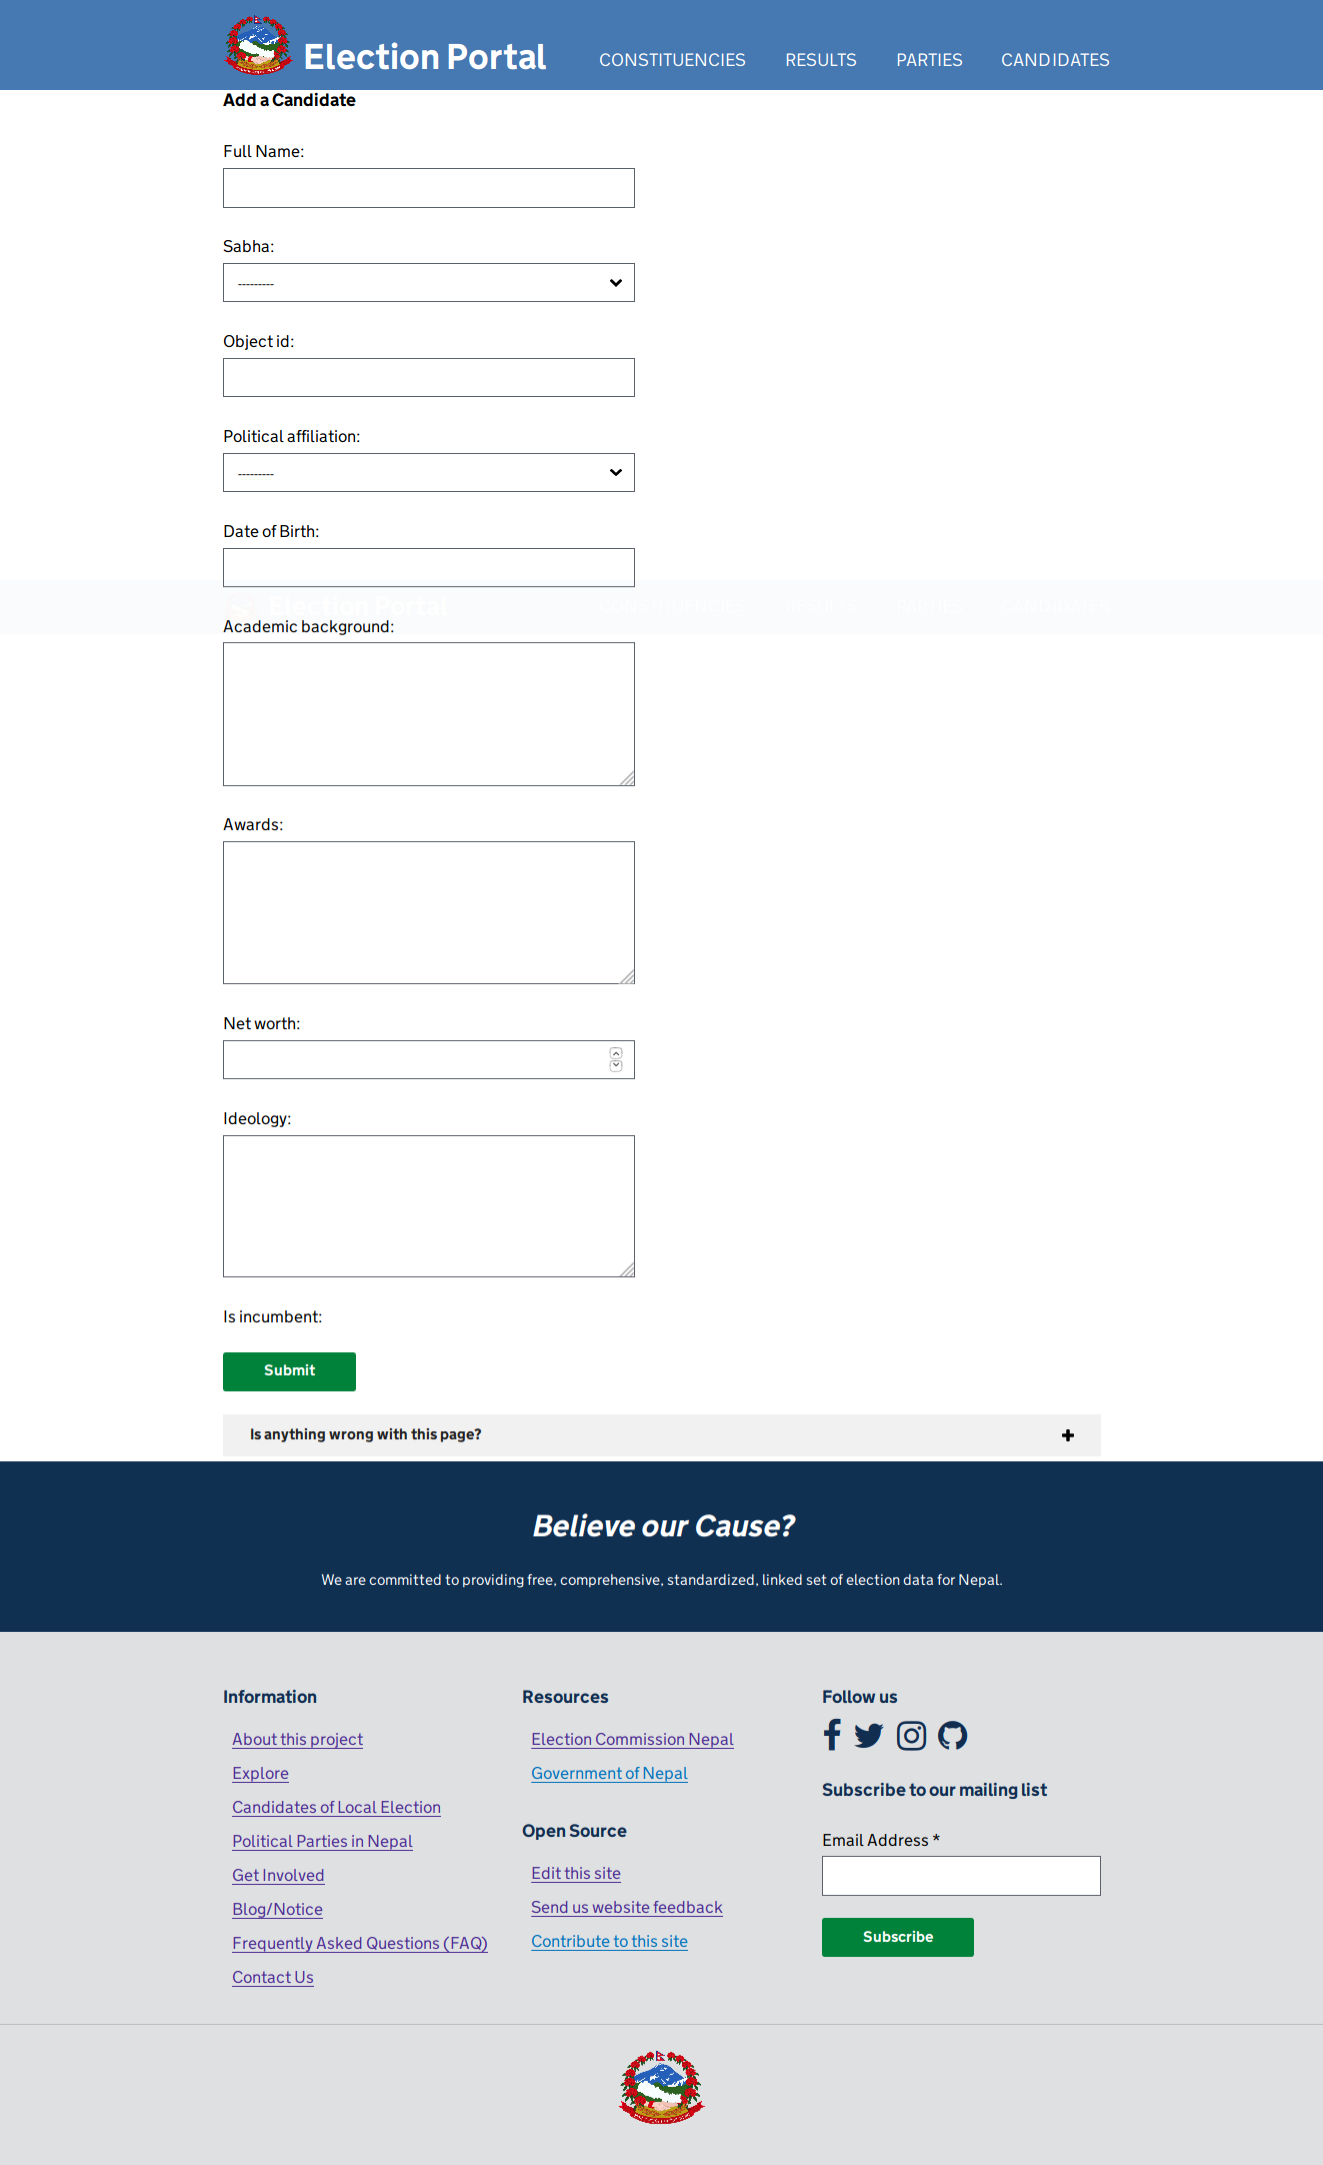
\includegraphics[scale=0.25]{Form_To_Add_Candidate.png}
\end{center}


\subsection{Form to Add Political Party}
\begin{center}
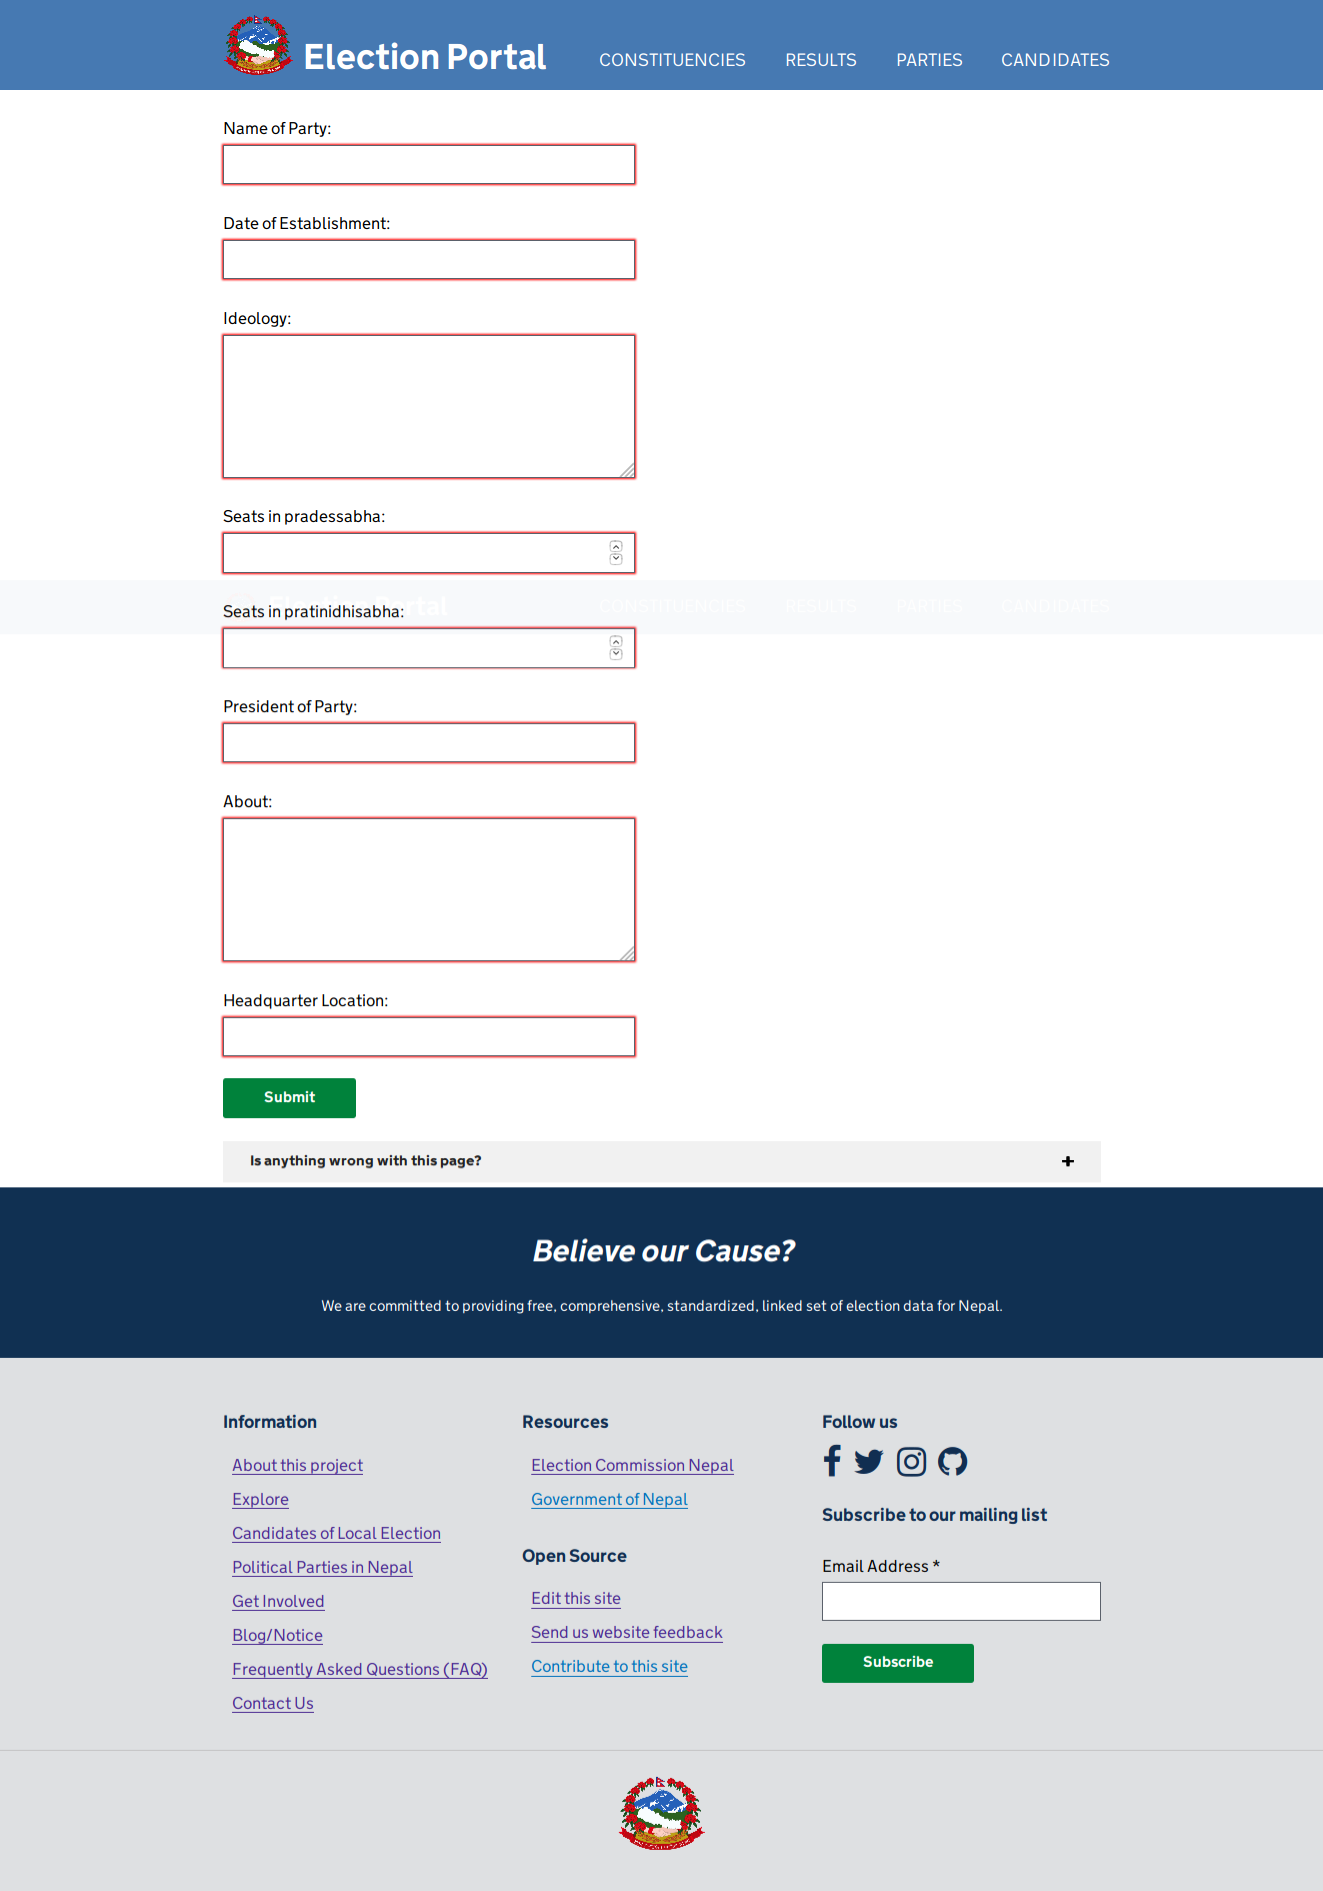
\includegraphics[scale=0.25]{Form_To_Add_Political_Party.png}
\end{center}


\subsection{Form To Add Province}
\begin{center}
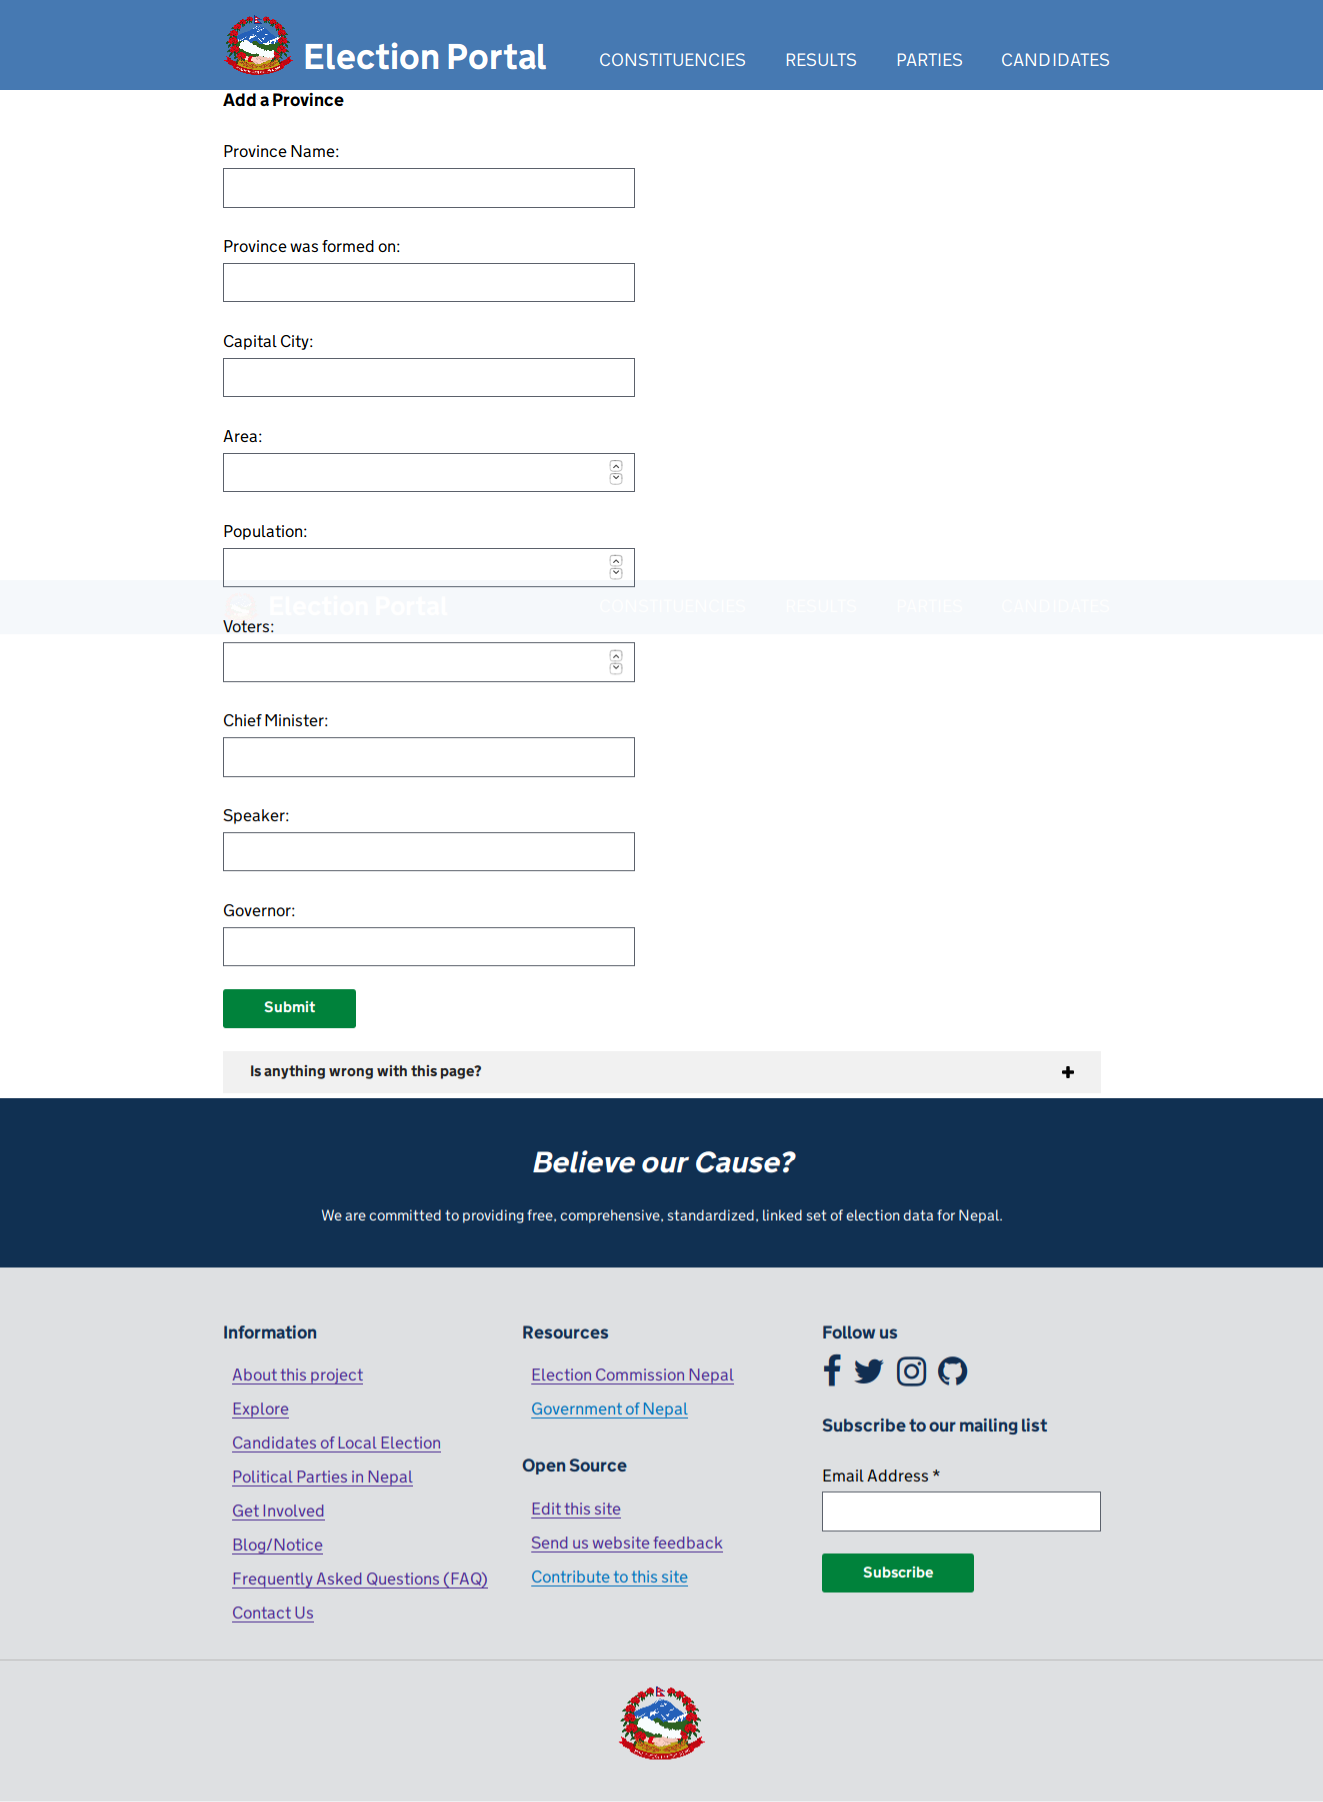
\includegraphics[scale=0.25]{Form_To_Add_Province.png}
\end{center}





\begin{thebibliography}{9}
 
\bibitem{UCD}
Wikipedia - Use Case Diagram
\\\texttt{https://en.wikipedia.org/wiki/Use-case-diagram}

\bibitem{CD}
Wikipedia - Class Diagram
\\\texttt{https://en.wikipedia.org/wiki/Class-diagram}

\bibitem{Project Report}
Fedrous - Web Design Report
\\\texttt{https://slideshare.net/ferdous/web-design-project-report}
 
\bibitem{Django Website} 
Django Documentation:,
\\\texttt{https://docs.djangoproject.com/en/2.0/}
\end{thebibliography}

\end{document}
         